\section{Optimize \& refactor code} \label{sec:optimize}
In section \ref{ssec:profiling_results} it is shown that the function \lstinline[language=c]|LineFinder::calculateNrPointsInEachBin| is the most time consuming function in all phases of the LUA software.

Before optimization can take place it is essential to understand the structure of this part of the LUA software. Algorithm \ref{alg:calculateNrPointsInEachBin} shows the pseudo code of the function \lstinline[language=c]|LineFinder::calculateNrPointsInEachBin|.

\begin{algorithm}
    \begin{algorithmic}[1]
        \Function{calculateNrPointsInEachBin}{$\alpha$}
        \State \textit{calculate sine and cosine of this angle} $\alpha$
        \State \textit{fetch X Z coordinates of the data points}
        \State \textit{fetch the indices of the data points (used to determine line association)}
        \State \textbf{for} \textit{each data point} \textbf{do}
        \State \hspace{1cm} \textit{check if data point is not already associated to a line}
        \State \hspace{1cm} \textit{calculate distance between data point and laser line scanner's origin}
        \State \hspace{1cm} \textit{determine in which distance bin a data point falls}
        \State \textbf{end for}
        \EndFunction
    \end{algorithmic}
    \caption{Pseudo code of the function \lstinline[language=c]|LineFinder::calculateNrPointsInEachBin|.}
    \label{alg:calculateNrPointsInEachBin}
\end{algorithm}

Algorithm \ref{alg:calculateNrPointsInEachBin} is nested in a loop that iterates over search angles specified for the Hough transform. This is shown in algorithm \ref{alg:binContainingMostPoints}

\begin{algorithm}
    \begin{algorithmic}[1]
        \Function{calculateBinContainingMostPoints}{}
        \State \textbf{for} \textit{each angle} $\alpha$ \textbf{in} \textit{all search angles} \textbf{do}
        \State \hspace{1cm} \textit{calculateNrPointsInEachBin}($\alpha$)
        \State  \hspace{1cm} \textbf{for} \textit{each distance bin} \textbf{in} \textit{all search bins} \textbf{do}
        \State \hspace{2cm} \textbf{if} \textit{bin contains more points than the current maximum} \textbf{then}
        \State \hspace{3cm} \textit{update the current maximum}
        \State \hspace{2cm} \textbf{end if}
        \State \hspace{1cm} \textbf{end for}
        \State \textbf{end for}
        \EndFunction
    \end{algorithmic}
    \caption{Pseudo code of the function \lstinline[language=c]|LineFinder::calculateBinContainingMostPoints|.}
    \label{alg:binContainingMostPoints}
\end{algorithm}

With regards to the order of for-loops, it is optimal to have a larger inner for-loop and a smaller outer for-loop \cite[lecture 7, "temporal locality" ]{scientific_programming}. Algorithms \ref{alg:calculateNrPointsInEachBin} and \ref{alg:binContainingMostPoints} show the nested for-loop structure that is used to perform the Hough transform. Note that the number of search angles is approximately 30, while the number of data points is approximately 4000. This means that the inner for-loop is much larger than the outer for-loop. Hence, the order of the for-loops is already optimal.

Closer inspection of algorithm \ref{alg:calculateNrPointsInEachBin} reveals that the fetching operations in lines 2 and 3 do not depend on the angle $\alpha$. This means that these fetching operations can be moved outside the for-loop. This ultimately results in less memory calls happening in the inner for-loop. Furtermore, the calculation of the sine and cosine can be done once for all angles in the main thread for of the LUA software before the main program loop (figure \ref{fig:code_flow}).

Figure \ref{fig:profiling_bottleneck_optimized} shows the profiling results of the implemented prefetching and precalculation optimizations.

\begin{figure}[H]
    \centering
    \begin{subfigure}{\textwidth}
        \centering
        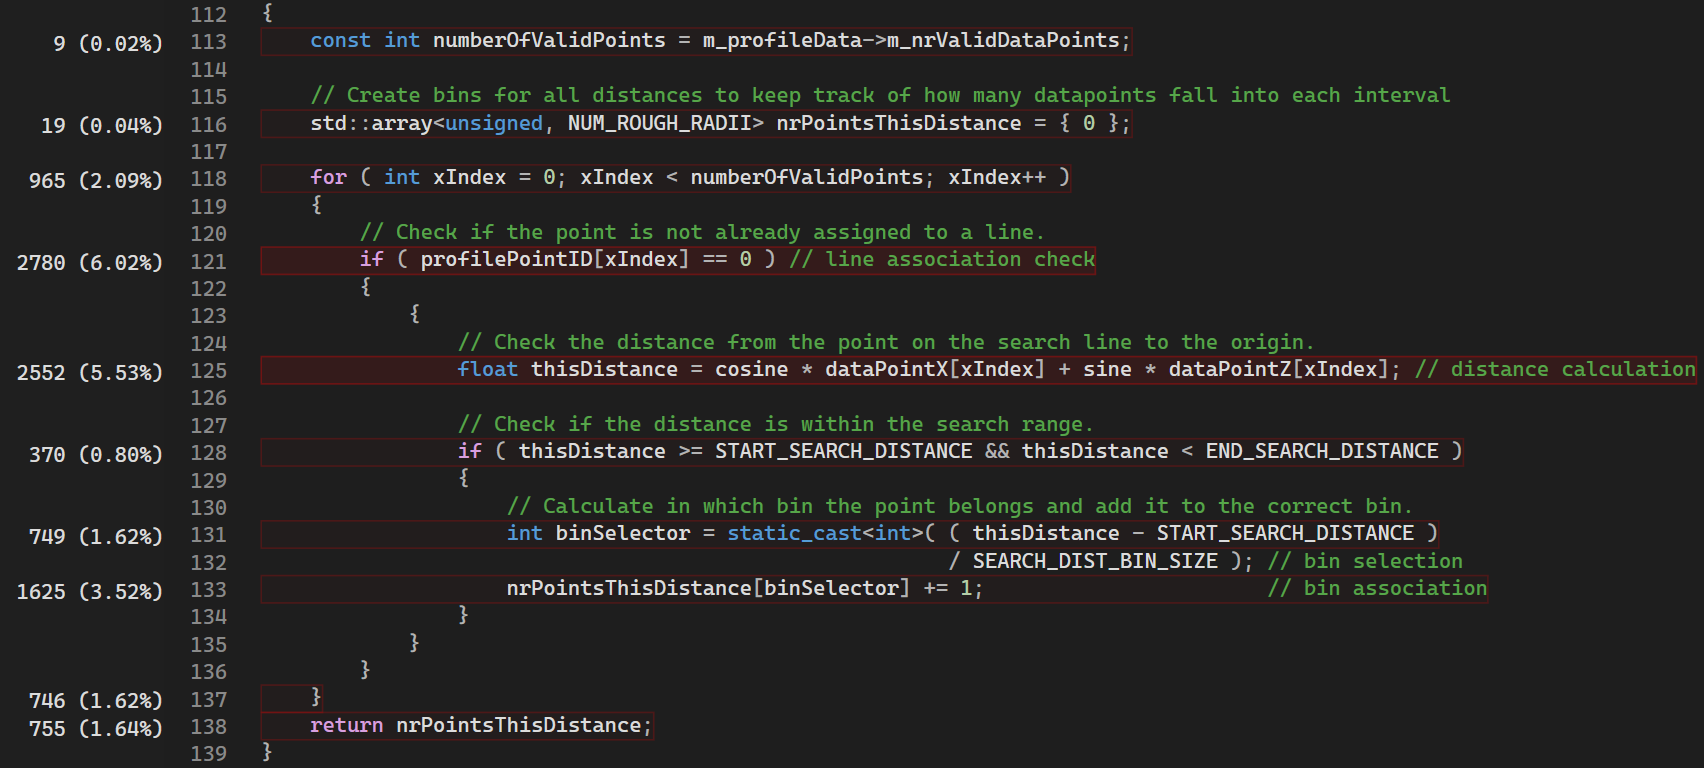
\includegraphics[width=\textwidth]{images/profiling_bottleneck_optimized.png}
        \caption{Profiling results of the function \lstinline[language=c]|LineFinder::calculateNrPointsInEachBin| (algorithm \ref{alg:calculateNrPointsInEachBin}) after precalculation optimization.}
    \end{subfigure}
    \begin{subfigure}{\textwidth}
        \centering
        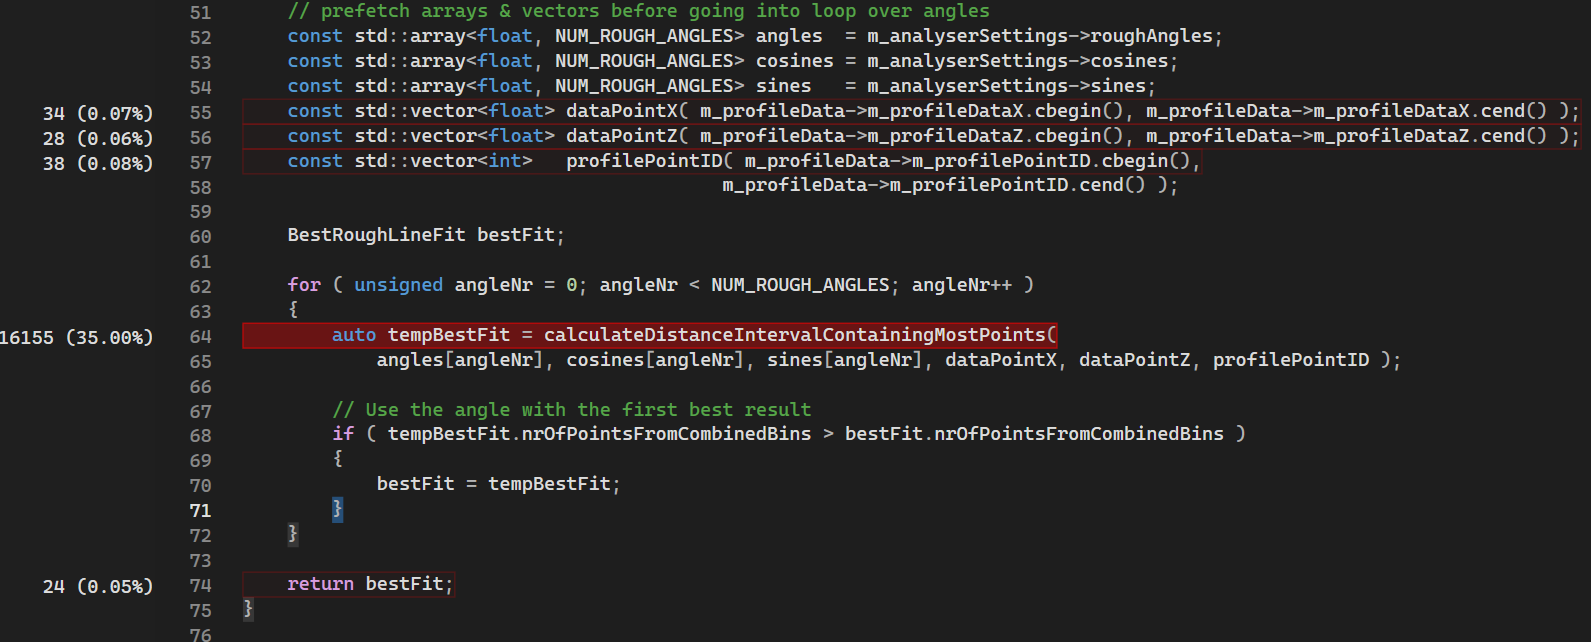
\includegraphics[width=\textwidth]{images/profiling_results_precalculation.png}
        \caption{Profiling results of the function \lstinline[language=c]|LineFinder::calculateBinContainingMostPoints| (algorithm \ref{alg:binContainingMostPoints}) after prefetching optimization.}\label{fig:profiling_results_precalculation}
    \end{subfigure}
    \caption{Profiling results of optimized bottleneck functions. Calculation of the sinusoidal functions is during initialisation of the LUA software. Data arrays are prefetched before the main loop.}
    \label{fig:profiling_bottleneck_optimized}
\end{figure}

Comparing lines 55-57 from figure \ref{fig:profiling_results_precalculation} with lines 81-84 from figure \ref{fig:profiling_bottleneck} shows that both the percentage of CPU time and the number of times these lines are sampled by the profiler are lower in the optimized case. This is a clear indication that the optimizations have been successful.

Further optimizations can be made by avoiding the most time consuming operation in the inner for-loop \ref{bottlen:line_assocation}. In general an if-statement in a for-loop causes a `pipeline stall' \cite[lecture 7, "Pipeline stall", slide 19]{scientific_programming}. This is because the CPU must wait until the if-statement is evaluated before it can continue executing the next instruction. This effect is made worse by the fact that the if-statement is in the inner most nested for-loop. The solution to this problem is to use a data structure that allows for fast look-up of data points that are already associated to a line. Perhaps this can be done by using a hash table. Alternatively, algorithmic adjustments can be made to avoid the if-statement entirely. In any case, this is left as a topic for future work.